\chapter{Theoretische Grundlagen}
Das Projekt basiert auf einigen theoretische Grundlagen. Dazu zählen
Lerntheorien und technische Begriffe, deren Erläuterungen Inhalt
dieses Kapitels sind. Dabei handelt es sich um eine Kurzfassung der
Beschreibungen aus \cite{gruben:2012}.

\section{Lernen}
Das Lernen selbst wird heute als ein Prozess verstanden. Dabei wirken "`mehrere
zentrale psychologische Phänomene (Motivation, Emotion,
Kognition)"'\cite{niegemann:2004} zusammen. 

Der Lernprozess besteht dabei aus drei Abschnitten:
\begin{enumerate}
  \item Zunächst werden Eindrücke wahrgenommen. Dabei tragen neue oder
  vergessene Eindrücke zur Umstrukturierung im Gehirn bei.
  \item Umstrukturieren bedeutet, dass Synapsen bewegt und andere Gehirnzellen
  angekoppelt werden.
  \item Mit Wiederholungen wird Wissen persistiert. Es entstehen stabile
  Strukturen, welche einfach und schnell abrufbar sind.
\end{enumerate}
In Abbildung \ref{pic:structSyn} wird diese Umstrukturierung illustriert
\cite{spitzer:2012}.

Von ein LMS wird erwartet, dass es diesen Lernprozess unterstützt. Anfänger
sollen die Möglichkeit erhalten zunächst klein anzufangen und die Grundlagen
eines bestimmten Sachverhaltes kennenzulernen. Fortschreitend können die
Anforderungen und Herausforderungen gesteigert werden, um den Lernprozess zu
unterstützten und zugleich die Motivation aufrecht zu erhalten.

\begin{figure}[H]
\centering
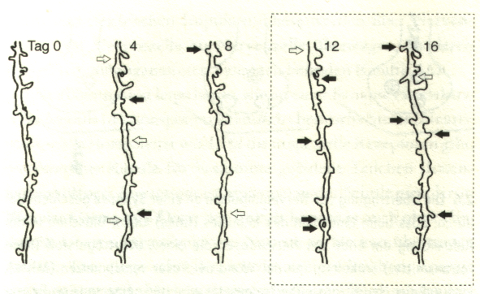
\includegraphics[width=0.7\textwidth]{SPIsynapseS50.png}
\caption{Umstrukturierung von Synapsen \footnotemark}\label{pic:structSyn}
\end{figure}\footnotetext{aus \cite{spitzer:2012}}

\section{Motivation}
Die Motivation ist ein wesentliches Standbein des Lernprozesses. Fehlt sie, so
ist es für Lernende bedeutend erschwert, Lerninhalte aufzunehmen, zu verarbeiten
und zu verstehen. Mithilfe von Motivation wird ein charakteristisches Verhalten
an den Tag gelegt, welches den Lernprozess aufrecht erhält \cite{jacobs:2010}.

Im Mittelpunkt jeder Motivation steht stets das persönliche Glück
\cite{stampfl:2012}. Dabei stehen Mittel zur Verfügung, die dem Lernenden auf
unterschliedliche weise unterstützen zu verstehen. Er kann zum einen
intrinsisch und zum anderen extrinsisch motiviert werden.

\subsection{Intrinsische Motivation}
Die intrinsische Motivation wird auch als direkte Motivation bezeichnet. Damit
wird der Lernende direkt angesprochen und in seinen Bedürfnissen befriedigt und
seinen Wünschen wird unmittelbar nachgegangen. Ein intrinsisch motivierter
Lernender geht einer Tätigkeit im eigenen Interesse nach, es sind keine externen
Einflüsse nötig, die ihn zu seinen Handlungen erst bewegen müssen
\cite{jacobs:2010}.

Jede Lernsoftware hat aus dem zuvor erwähnten Sachverhalt die intrinsiche
Motivation zum Ziel. Dazu werden nicht selten unter Anderem auch gamifizierende
Inhalte verwendet (siehe \ref{ref:gamification}).

\subsection{Extrinsische Motivation}
Die andere Seite der Motivation kommt von aussen. Es werden Belohnungen gegeben
oder Strafe und negative Konsequenzen vermieden. Synonyme sind demnach
"`indirekte Motivation"', das "`Butterbrot-und-Peitsche-Prinzip"' oder
"`Manipulation"' \cite{jacobs:2010}.

Für Masterly Mate im Speziellen, kann der Tutor ein extrinsisch Motivierender
Faktor sein. Hinzu kommen die gamifizierenden Elemente der zu erreichenden
Punktzahl pro WBT und das Aufsteigen in Rängen. Implizit wird auch Strafe in der
Form angewandt, dass es laut Konzept auch möglich ist, im Rang zu fallen
(siehe dazu Tabelle \ref{tab:privilegesRoles}).

\section{Lernmodelle}
Zum Zweck der Unterstützung des Lernprozesses und Förderung der Motivation haben
sich einige Lernmodelle herauskristallisiert, die heute als gültig und
vertretbar angesehen werden. In der Idee von MasterlyMate sind explizit zwei
Lernmodelle verwoben. Das Dreyfus fünf Etappen Modell mentaler Aktivitäten und
Blended Learning.

\subsection{Das Dreyfus fünf Etappen Modell mentaler
Aktivitäten}\label{ref:dreyfus}
Inhalt des Dreyfus-Modells ist das Hinterfragen, welche Person einer anderen
einen bestimmten Sachverhalt erklären sollte. Dabei wird insbesondere
berücksichtigt, wie groß der Unterschied der Fachkompetenz zwischen Lernenden
und Lehrenden ist. Es wurden insgesamt fünf Ränge\footnote{Novice, Competence,
Proficiency, Expertise, Mastery} definiert, die den Lernweg von abstrakten
Prinzipien hin zu konkreter Erfahrung mit der Aneignung von Wissen beschreiben
\cite{dreyfus:1980}.

Allgemein formuliert sollte kein Experte einem Neuling etwas erklären. Steigt
man neu in ein Fachgebiet ein, so sind zunächst simple und einfache Beispiele
verbunden mit einem engen Betrachtungswinkel des Sachverhalts sehr hilfreich.
Ein Experte würde den Neuling mit unnötigen Details überhäufen.

Dazu staffelt sich der Lernerfolg in fünf Etappen:
\begin{description}
  \item[1. Novize] Ein Novize ist auf grundlegende Anweisungen angewiesen. Er
  verfügt über kein Vorwissen und evaluiert sich nicht selbst. Mit extrinsischem
  Feedback wird dem Abkommen vom Regelwerk zuvorgekommen.
  \item[2. Fortgeschrittener] Die Handlungen des Fortgeschrittene sind gegenüber
  dem Novizen weniger kontextfrei. Sein weiterer Lernweg kann auf seiner kleinen
  Wissensbasis aufbauen. Er hat grundlegende Prinzipien verstanden und erkennt
  situationsbasierte Muster. Der Fortgeschrittene kann simple Beispiele anhand
  von Guidelines durchlaufen, er experimentiert jedoch nicht.
  \item[3. Erfahrener] Der Umgang mit typischen Situationen am ihm gegebenen
  System stellen keine Hürden für den Erfahrenen dar. Ihm ist es möglich neue
  Situationen anzuknüpfen, einzuordnen und sehr ähnliche bewusst zu
  unterscheiden. Der Erfahrene arbeitet nach selbst erschaffenen Maximen.
  \item[4. Experte] Der Experte ist kein geeigneter Lehrer für einen Novizen
  mehr. Er hat die grundlegenden Prinzipien verloren und arbeitet nach seiner
  Intuition, einer Mischung aus Regeln, Guidelines und Maximen. Lösungen für
  ungewohnte Situationen gehören stets zum Reportoir des Experten. Im Sinne der
  fachlichen Kompetenz ist dieser Grad der höchste.
  \item[5. Meister] Ein Meister zeichnet sich gegenüber dem Experten neben
  fachlicher Kompetenz durch herausragende didaktische Fähigkeiten aus. Er
  bleibt damit auch ein geeigneter Lehrer für Novizen.
\end{description}

Generell sollte sich ein Lehrer zwei Grade über seinem Schüler befinden oder
Meister sein. Weitere detailliertere Erklärungen zu den Rängen finden sich in
\cite{gruben:2012}.

\subsection{Blended Learning}\label{ref:blendedLearning}
Zweck des Blended Learning, zu deutsch auch Integriertes Lernen genannt, ist das
Verschmelzen der Vorteile diverser Lernformen. Darunter befinden sich
\ac{F2F}-Education, \ac{DE} und \ac{OE} (eLearning). Die jeweiligen Nachteile
wurden dabei weitestgehend überwunden \cite{kroeger:2004}.

MasterlyMate verfolgt die Verschmelzung von F2F-Education, der Durchführung von
Präsenzunterricht, mit eLearing, dem Durcharbeiten von WBTs. Die DE wird dabei
nur am Rande betrachtet, da nur in Ausnahmefällen Unterweisungen über Chats oder
ähnliche Kommunikationskanäle vonstatten gehen sollen.

\section{eLearning}


\section{Gamification}\label{ref:gamification}